\documentclass[border=4pt]{standalone}
\usepackage{pgfplots}
\pgfplotsset{compat=1.18}

\begin{document}
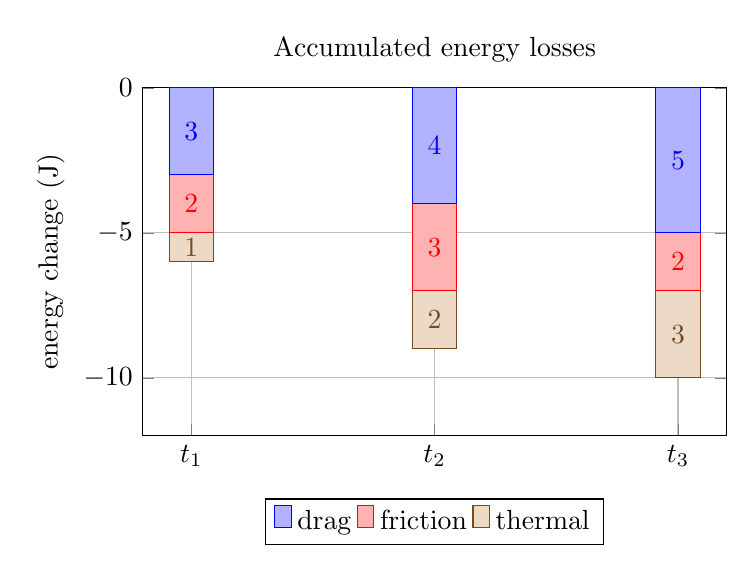
\begin{tikzpicture}
  \begin{axis}[
    ybar stacked=minus,
    stack negative=on previous,
    width=9cm,
    height=6cm,
    bar width=16pt,
    ymin=-12,
    ymax=0,
    xtick={1,2,3},
    xticklabels={$t_1$,$t_2$,$t_3$},
    ylabel={energy change (J)},
    title={Accumulated energy losses},
    grid=major,
    nodes near coords,
    legend style={at={(0.5,-0.18)},anchor=north,legend columns=-1}
  ]
    \addplot coordinates {(1,3) (2,4) (3,5)};
    \addplot coordinates {(1,2) (2,3) (3,2)};
    \addplot coordinates {(1,1) (2,2) (3,3)};
    \legend{drag,friction,thermal}
  \end{axis}
\end{tikzpicture}
\end{document}
